\documentclass[a4paper,12pt]{article}
\usepackage{graphicx} 
\usepackage{amsmath} 

\usepackage{indentfirst}
\usepackage{amsmath} 
\usepackage[varg]{txfonts}
\usepackage{colortbl}
\topmargin=-0.75cm
\oddsidemargin=0.0cm
\evensidemargin=0.0cm



\definecolor{LemonChiffon}{rgb}{1.,0.98,0.8}
\definecolor{Gold}{rgb}{1.,0.84,0.}
\definecolor{darkblue}{rgb}{0.25,0.,0.95}
\definecolor{lightblue}{rgb}{0.4,0.65,0.95}
\definecolor{grayred}{rgb}{0.7,0.,0.} 
\definecolor{red2}{rgb}{1.0,0.5,0.} 
\definecolor{LemonChiffon}{rgb}{1.,0.98,0.8}
\definecolor{Gold}{rgb}{1.,0.84,0.}
\definecolor{darkblue}{rgb}{0.25,0.,0.95}
\definecolor{lightblue}{rgb}{0.4,0.65,0.95}
\definecolor{RGBblack}{rgb}{0.0,0.0,0.0} 
\def\red{\color{red}}
\def\green{\color{green}}
\def\white{\color{white}}
\def\white{\color{LemonChiffon}}
\def\blue{\color{lightblue}}
\def\gold{\color{Gold}}
\def\black{\color{RGBblack}}



\def\pp{\mathaccent "7F }
\def\p{\mathaccent 95 }


\def\sini {\sin i}
\def\cosi {\cos i}

\def\sino {\sin \Omega}
\def\coso {\cos \Omega}
\def\sinw {\sin \omega}
\def\cosw {\cos \omega}



\begin{document}
\font\norm=cmr12
\font\hugeb=cmb22
\font\isob=cmb18
\font\iso=cmr18
\font\med=cmr14
\font\medb=cmb14
\baselineskip 0.6cm
\parskip\medskipamount
\parskip 0.2cm
\parindent 5mm

%\boldmath

\norm
\hsize 16cm
\vsize 30cm
\newcommand{\bul}{$\bullet \ \ $}
\newcommand{\buu}{\hskip 0.5cm}
\newcommand{\arrow}{$\Rightarrow \ \ $}
\newcommand{\barrow}{\hskip 0.5cm $\Rightarrow \ \ $}
\newcommand{\larrow}{\hskip 0.5cm $\Leftarrow \ \ $}
\newcommand{\hlin}{\vskip 0.5cm}
\newcommand{\hpar}{\vskip 1.0cm}
\newcommand{\nin}{\noindent}
\def\pii{\tilde{\omega}_\circ}

\newcommand{\VV}{$\vec V$ \hskip 0.1cm}
\newcommand{\RR}{$\vec R$ \hskip 0.1cm}

\newcommand{\VVE}{\vec V}
\newcommand{\RRE}{\vec R}

\newcommand{\sverb}{\begin{verbatim}}
\newcommand{\everb}{\end{verbatim}}


%\pagestyle{empty}
{\centerline{}




{\norm
\vskip 0cm
{{\centerline { {\isob CELESTIAL MECHANICS (Fall 2012): }}}}
\vskip 0.2cm
{{\centerline { {\isob COMPUTER EXERCISES I - SOLUTIONS}}}}

{{\centerline { { (Heikki Salo 05.10.2012)}}}}

\vskip 2cm
{\medb 1. Solution of Kepler's equation}

{\medb 2. Study elliptical orbits}

{\medb 3. Compare different anomalies: $E$, $f$, $M$}

{\medb 4. Numerical evaluation of time averages on elliptical orbit}


\newpage

\black

{\isob 1. Solution of Kepler's equation}

\vskip 0.35cm

\framebox{\bf kepler.pro}

\bul Use always plenty of comments to document the code

\bul Actual variables (input M, KS; output E) transferred via call parameters, 

\buu control of optional output via keywords

\bul In-built info:  enter {\red kepler } to IDL propt to get info





{\red \scriptsize
\begin{verbatim}

;****************************************************************************
;	RATKAISTAAN KEPLERIN YHTALOSTA EKSENTRINEN ANOMALIA E
;	ITEROIMALLA KESKIANOMALIASTA M
;	RADAN EKSENTRISYYS = EKS
;****************************************************************************

	pro kepler,m,eks,e,itul=itul,itemax=itemax,check=check,tole0=tole0

;****************************************************************************
 if(n_params() le 0) then begin
   print,'---------------------------------------------'
   print,' kepler,M,eks,E'
   print,'---------------------------------------------'
   print,' SOLVES KEPLER-EQUATION M = E - eks*sin(E)' 
   print,' USING SUBSTITUTION ITERATION'
   print,' input:   M = mean anomaly (in radians), eks=eccentricity '
   print,' output:  E = eccentric anomaly (in radians)'
   print,' keywords: '
   print,'   /itul  -> output iteration values (E)'
   print,'   /check -> check accuracy of solution'
   print,'   itemax =  max number of iterations (def=500)'
   print,'   tole   =  desired accuracy  (def=1d-10)'
   print,' example:  eks=0.5, M= 45 degrees, output iteration values'
   print,"   kepler,45./!radeg,0.5,e,/itul & print,'E=',e*!radeg,' deg'"
   print,'   HS 04.10.02/01.11.2006/10.11.2008'
   print,'---------------------------------------------'
   return
 endif

;****************************************************************************
; solve eccentric anomaly E from mean anomaly M, for eccentricity EKS
; using substitution iteration
;  M= E - eks*sin(E)  -> E = M + eks*sin(E)
; iteration: 
;  E_OLD = M + eks * sin(M)/(1-eks*cos(M))  first guess
;  E_NEW = M + eks * sin(E_OLD)             until abs(E_NEW-E_OLD) < tole
;****************************************************************************

	nstep=500
	if(keyword_set(itemax)) then nstep=itemax
        tole=1d-10
	if(keyword_set(tole0)) then tole=tole0
	i=0
	e=m+eks*sin(m)/(1.d0-eks*cos(m))

\end{verbatim}
\black}

{\red \scriptsize
\begin{verbatim}
	if(keyword_set(itul)) then begin
	  print,' M   = ',m*!radeg,' degrees'
	  print,' EKS = ',eks
          print,'      step      E (rad)         E(deg)         dE(deg) '
          print,i,e,e*!radeg
	endif
	for i=1,nstep do begin
	    e_new=m+eks*sin(e)
            de=e_new-e
	    e=e_new
	    if(keyword_set(itul)) then print,i,e,e*!radeg,de*!radeg
	    if(abs(de) lt tole) then goto,end_ite
	endfor
	end_ite: 
        if(keyword_set(check)) then $
           print,'M - (E-eks*sin(E)) =',m-(e-eks*sin(e))
        return
	end
;***********************************************************************
\end{verbatim}
\black}


\framebox{{\bf kepler\_demo.pro}}

\bul Example of calling kepler.pro: how many iterations
are needed to reach the accuracy of $0.01^\circ$, when $M= 45^\circ$,
and $\epsilon =0.01, \ 0.05, \ 0.50, \ 0.90, \ 0.99$.

\buu (try also $M=359^\circ$!)

{\red \scriptsize \begin{verbatim}

;***************************************
;kepler\_demo.pro (HS 2002/1.11.2006)
;***************************************
;use kepler.pro for solving E for M=45 degrees
;with accuracy of 0.001 degrees
;for eccentricities 0.01, 0.05, 0.50, 0.90, 0.99
;kepler.pro: use without arguments -> prints info

M=45./!radeg         ; !radeg = system variable 180/pi
;M=359./!radeg        ; try also this
tole=0.01/!radeg

print,'----------------------------------------'
kepler,M,0.01,e,/itul,tole=tole
print,'----------------------------------------'
kepler,M,0.05,e,/itul,tole=tole
print,'----------------------------------------'
kepler,M,0.50,e,/itul,tole=tole
print,'----------------------------------------'
kepler,M,0.90,e,/itul,tole=tole                   
print,'----------------------------------------'
kepler,M,0.99,e,/itul,tole=tole                   
print,'----------------------------------------'
end

\end{verbatim}} \black



\newpage

\bul Output from {\bf kepler\_demo.pro} 

{\scriptsize \begin{verbatim}
----------------------------------------
IDL> .run kepler_demo
% Compiled module: $MAIN$.
----------------------------------------
 M   =       45.0000 degrees
 EKS =    0.01000000
      step      E (rad)         E(deg)         dE(deg) 
       0      0.79251961       45.408026
       1      0.79251943       45.408016  -1.0284570e-05
----------------------------------------
 M   =       45.0000 degrees
 EKS =     0.0500000
      step      E (rad)         E(deg)         dE(deg) 
       0      0.82204934       47.099955
       1      0.82202531       47.098578   -0.0013770682
----------------------------------------
 M   =       45.0000 degrees
 EKS =      0.500000
      step      E (rad)         E(deg)         dE(deg) 
       0       1.3323163       76.336099
       1       1.2712473       72.837099      -3.4989995
       2       1.2631330       72.372187     -0.46491248
       3       1.2619201       72.302691    -0.069495718
       4       1.2617361       72.292148    -0.010542862
       5       1.2617081       72.290545   -0.0016029152
----------------------------------------
 M   =       45.0000 degrees
 EKS =      0.900000
      step      E (rad)         E(deg)         dE(deg) 
       0       2.5356433       145.28165
       1       1.2979865       74.369147      -70.912507
       2       1.6521140       94.659156       20.290010
       3       1.6824241       96.395798       1.7366413
       4       1.6797966       96.245252     -0.15054518
       5       1.6800570       96.260169     0.014916224
       6       1.6800315       96.258706   -0.0014621270
----------------------------------------
 M   =       45.0000 degrees
 EKS =      0.990000
      step      E (rad)         E(deg)         dE(deg) 
       0       3.1191281       178.71287
       1      0.80763619       46.274142      -132.43873
       2       1.5008269       85.991045       39.716903
       3       1.7729758       101.58403       15.592980
       4       1.7552331       100.56745      -1.0165799
       5       1.7586075       100.76078      0.19333613
       6       1.7579893       100.72536    -0.035419300
       7       1.7581034       100.73190    0.0065363228
----------------------------------------


\end{verbatim}} \black



\newpage
\black

{\isob 2. Study elliptical orbits} \framebox{elliptic\_demo.pro}

{\scriptsize \red \begin{verbatim}
;**********************************************
;elliptic_demo.pro
;study elliptic orbit
;HS 05.11.02/01.11.2006
;**********************************************
;A plot elliptic orbit using E
;B plot elliptic orbit using f
;C plot elliptic orbit using M
;D plot elliptic orbit using M,
;       plotting points with equal spacing in time
;E plot V, V_r, V_t
;F plot EKIN, EPOT, ETOT, AMOM

;*************************************
;plot elliptic orbits
;with eccentricity 0.1,0.2,...,0.8
;choose a=1. semimajor axis
;*************************************
  a=1.
;eccentricity values
  eks_tab=[0., 0.1, 0.2, 0.3, 0.4, 0.5, 0.6, 0.7, 0.8]
;make 4 plots on the same page
  !p.multi=[0,2,2]
;open new window
  nwin

;----------------------------------------------
; A)  use eccentric anomaly E as a parameter
;----------------------------------------------
  e=findgen(201)/200.*2.*!dpi
  sine=sin(e) &  cose=cos(e)
;loop over eccentricity values
  for i=0,n_elements(eks_tab)-1 do begin
     eks=eks_tab(i)
     b=sqrt(1.-eks^2)*a
     xx=a*(cose-eks)
     yy=b*sine
;i=0 plot, otherwise oplot
    if(i eq 0) then begin
      plot,xx,yy,xtitle='x',ytitle='y',xrange=[-2,2],yrange=[-2,2],$
           xs=1,ys=1,/iso,title='E as free parameter'
      plots,0,0,psym=1
    endif
    oplot,xx,yy,col=i+2
  endfor
  xyouts,-1.8,1.7,'eks=0.0, 0.1, ..., 0.8'

;----------------------------------------------
; B) use true anomaly f as a parameter
;----------------------------------------------
  f=findgen(201)/200.*2.*!dpi
  sinf=sin(f) &  cosf=cos(f)
  for i=0,n_elements(eks_tab)-1 do begin
    eks=eks_tab(i)
    p=(1.-eks^2)*a
    r=p/(1.+eks*cosf)
    xx=r*cosf
    yy=r*sinf
    if(i eq 0) then begin
      plot,xx,yy,xtitle='x',ytitle='y',xrange=[-2,2],yrange=[-2,2],$
           xs=1,ys=1,/iso,title='f as free parameter'
      plots,0,0,psym=1
    endif
    oplot,xx,yy,col=i+2
  endfor

;----------------------------------------------
; C) use mean anomaly M as a parameter
; requires solution of eccentric anomaly from Kepler's equation
; M = E - eks*sin(E)
;----------------------------------------------
  M=findgen(201)/200.*2.*!dpi
  for i=0,n_elements(eks_tab)-1 do begin
    eks=eks_tab(i)
    b=sqrt(1.-eks^2)*a
;solve kepler's equation for each M
    e=m*0
    for j=0,n_elements(m)-1 do begin
      kepler,m(j),eks,eano
      e(j)=eano
    endfor
    xx=a*(cos(e)-eks)
    yy=b*sin(e)
    if(i eq 0) then begin
       plot,xx,yy,xtitle='x',ytitle='y',xrange=[-2,2],yrange=[-2,2],$
            xs=1,ys=1,/iso,title='M as free parameter'
       plots,0,0,psym=1
     endif
    oplot,xx,yy,col=i+2
  endfor

;----------------------------------------------
; D) use mean anomaly M as a parameter
;    plot each point by symbol, otherwise as C)
;    to show how speed varies
;----------------------------------------------
;eccentricity values
  eks_tab=[0., 0.8]
  nwin
  M=findgen(101)/100.*2.*!dpi
  for i=0,n_elements(eks_tab)-1 do begin
    eks=eks_tab(i)
    b=sqrt(1.-eks^2)*a
    e=m*0
    for j=0,n_elements(m)-1 do begin
      kepler,m(j),eks,eano
      e(j)=eano
    endfor
    xx=a*(cos(e)-eks)
    yy=b*sin(e)
    if(i eq 0) then begin
      plot,xx,yy,xtitle='x',ytitle='y',xrange=[-2,2],yrange=[-2,2],$
           xs=1,ys=1,/iso,title='M as free parameter, eks=0.0 and 0.8',psym=3
      plots,0,0,psym=1
    endif
    oplot,xx,yy,col=i+2,psym=3
  endfor
;**********************************************************
 xyouts,0.01,0.01,'elliptic_demo.pro: page 1: a)-d)',/normal,chars=.75
 !p.multi=0
;**********************************************************

\end{verbatim} \black

\vspace{-17cm}
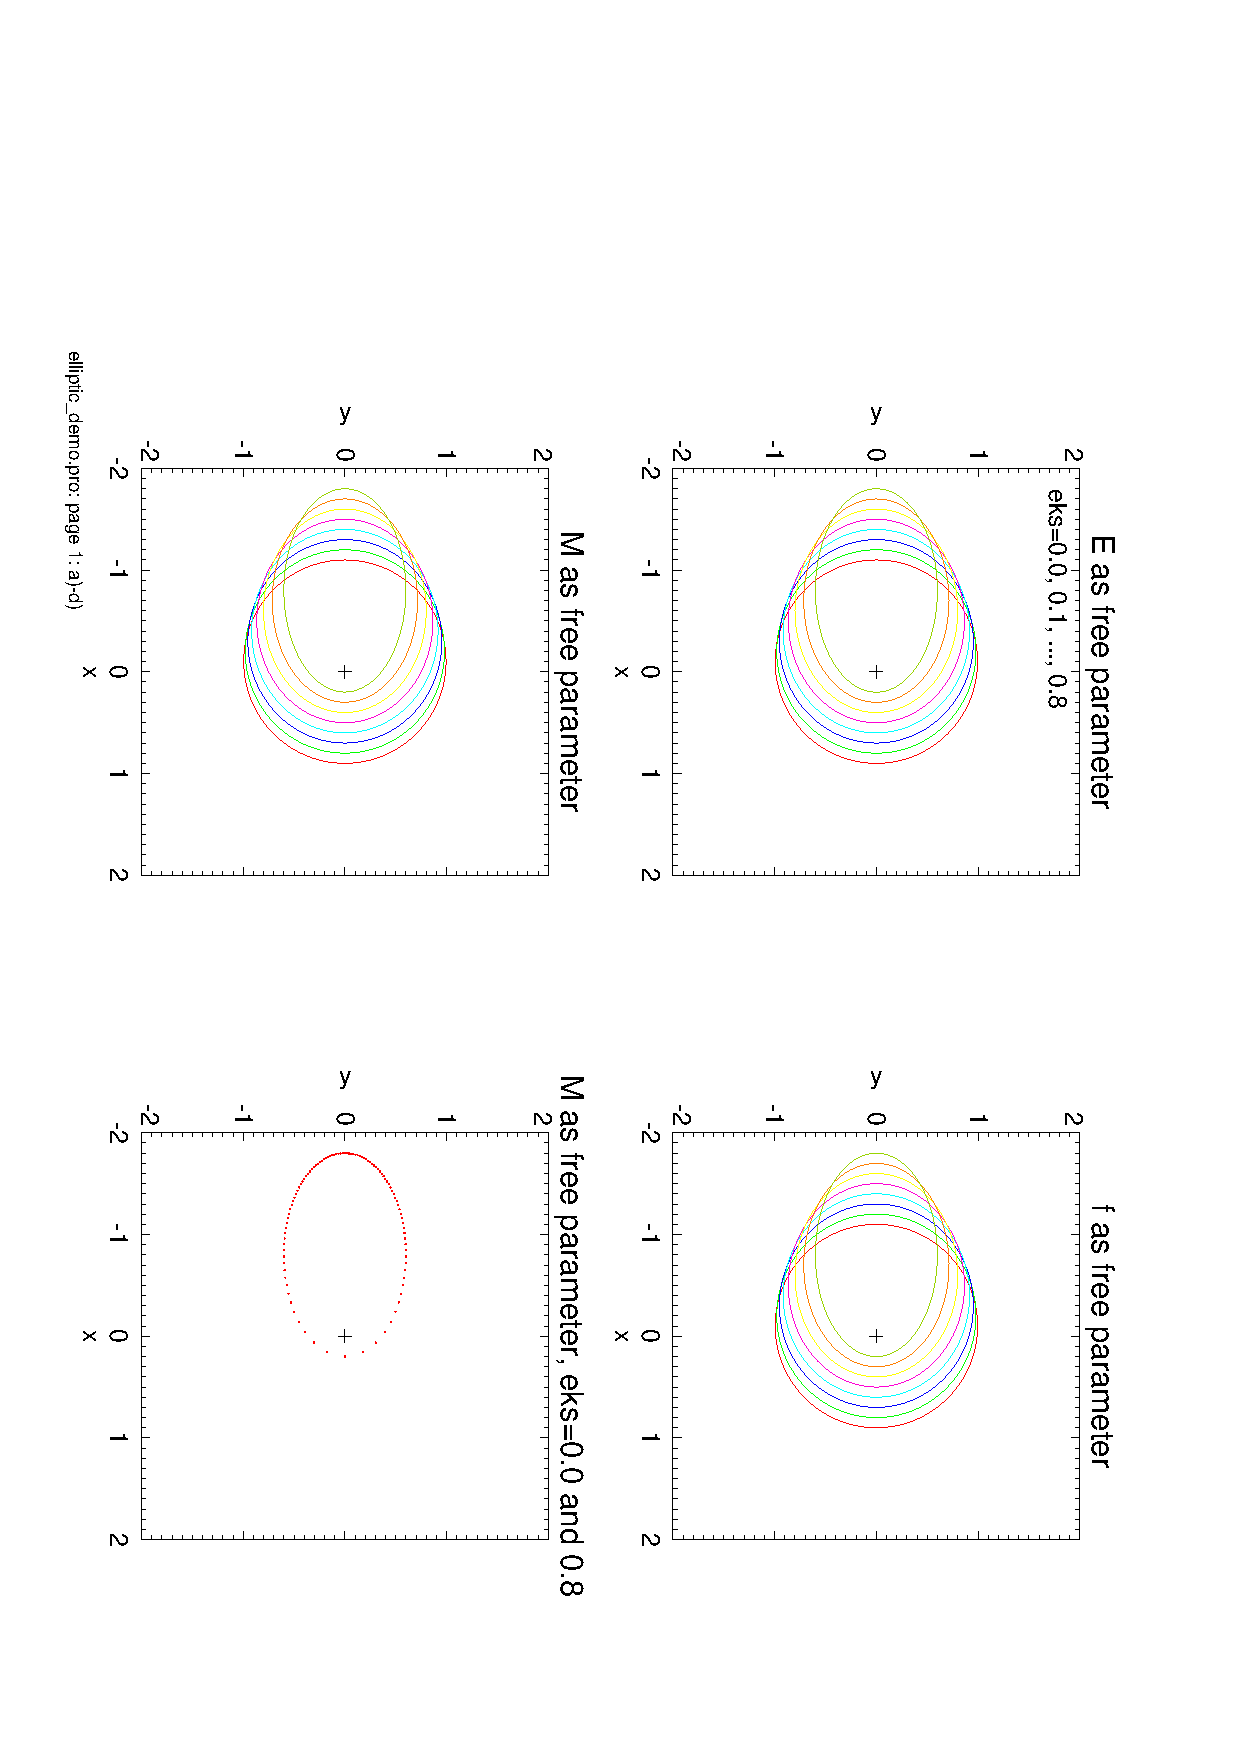
\includegraphics[width=1.1\paperwidth,height=1.1\paperheight]{elliptic_demo_1.pdf}
\clearpage

%********************************************************

{\red \scriptsize
\begin{verbatim}
;----------------------------------------------
; e) PLOT r, 1/r^2, 1/r^3 vs. TIME
;----------------------------------------------
!p.multi=[0,1,3]
nwin
!p.charsize=1.75
;eccentricity values
  eks_tab=[0., 0.4, 0.8]
  M=findgen(801)/400.*2.*!dpi

;---------- 
; r(t)
;---------- 
  for i=0,n_elements(eks_tab)-1 do begin
    eks=eks_tab(i)
    b=sqrt(1.-eks^2)*a
    e=m*0
    for j=0,n_elements(m)-1 do begin
      kepler,m(j),eks,eano
      e(j)=eano
    endfor
    rr=a*(1-eks*cos(e))
    if(i eq 0) then begin
      plot,m/2/!pi,rr,xtitle='T/PER',ytitle='r',xrange=[0,2],yrange=[0,2],$
           xs=1,ys=1,title='r vs time, eks=0.0, 0.4, 0.8',psym=3
    endif
    oplot,m/2/!pi,rr,col=i+2,psym=3
  endfor

;---------- 
; r(t)^(-2)
;---------- 
  for i=0,n_elements(eks_tab)-1 do begin
    eks=eks_tab(i)
    b=sqrt(1.-eks^2)*a
    e=m*0
    for j=0,n_elements(m)-1 do begin
      kepler,m(j),eks,eano
      e(j)=eano
    endfor
    rr=a*(1-eks*cos(e))
    if(i eq 0) then begin
      plot,m/2/!pi,1/rr^2,xtitle='T/PER',ytitle='1/r^2',$
           xrange=[0,2],yrange=[0,20],$
           xs=1,ys=1,title='r vs time, eks=0.0, 0.4, 0.8',psym=3
    endif
    oplot,m/2/!pi,1/rr^2,col=i+2,psym=3
  endfor

;---------- 
; r(t)^(-3)
;---------- 
  for i=0,n_elements(eks_tab)-1 do begin
    eks=eks_tab(i)
    b=sqrt(1.-eks^2)*a
    e=m*0
    for j=0,n_elements(m)-1 do begin
      kepler,m(j),eks,eano
      e(j)=eano
    endfor
    rr=a*(1-eks*cos(e))
    if(i eq 0) then begin
      plot,m/2/!pi,1/rr^3,xtitle='T/PER',ytitle='1/r^3',$
           xrange=[0,2],yrange=[0,200],$
           xs=1,ys=1,title='r vs time, eks=0.0, 0.4, 0.8',psym=3
    endif
    oplot,m/2/!pi,1/rr^3,col=i+2,psym=3
  endfor

;**********************************************************
 xyouts,0.01,0.01,'elliptic_demo.pro: page 2: e)',/normal,chars=.75
 !p.multi=0
 !p.charsize=1.
 charsize,1
 ;**********************************************************

\end{verbatim} \black

\vspace{-12cm}
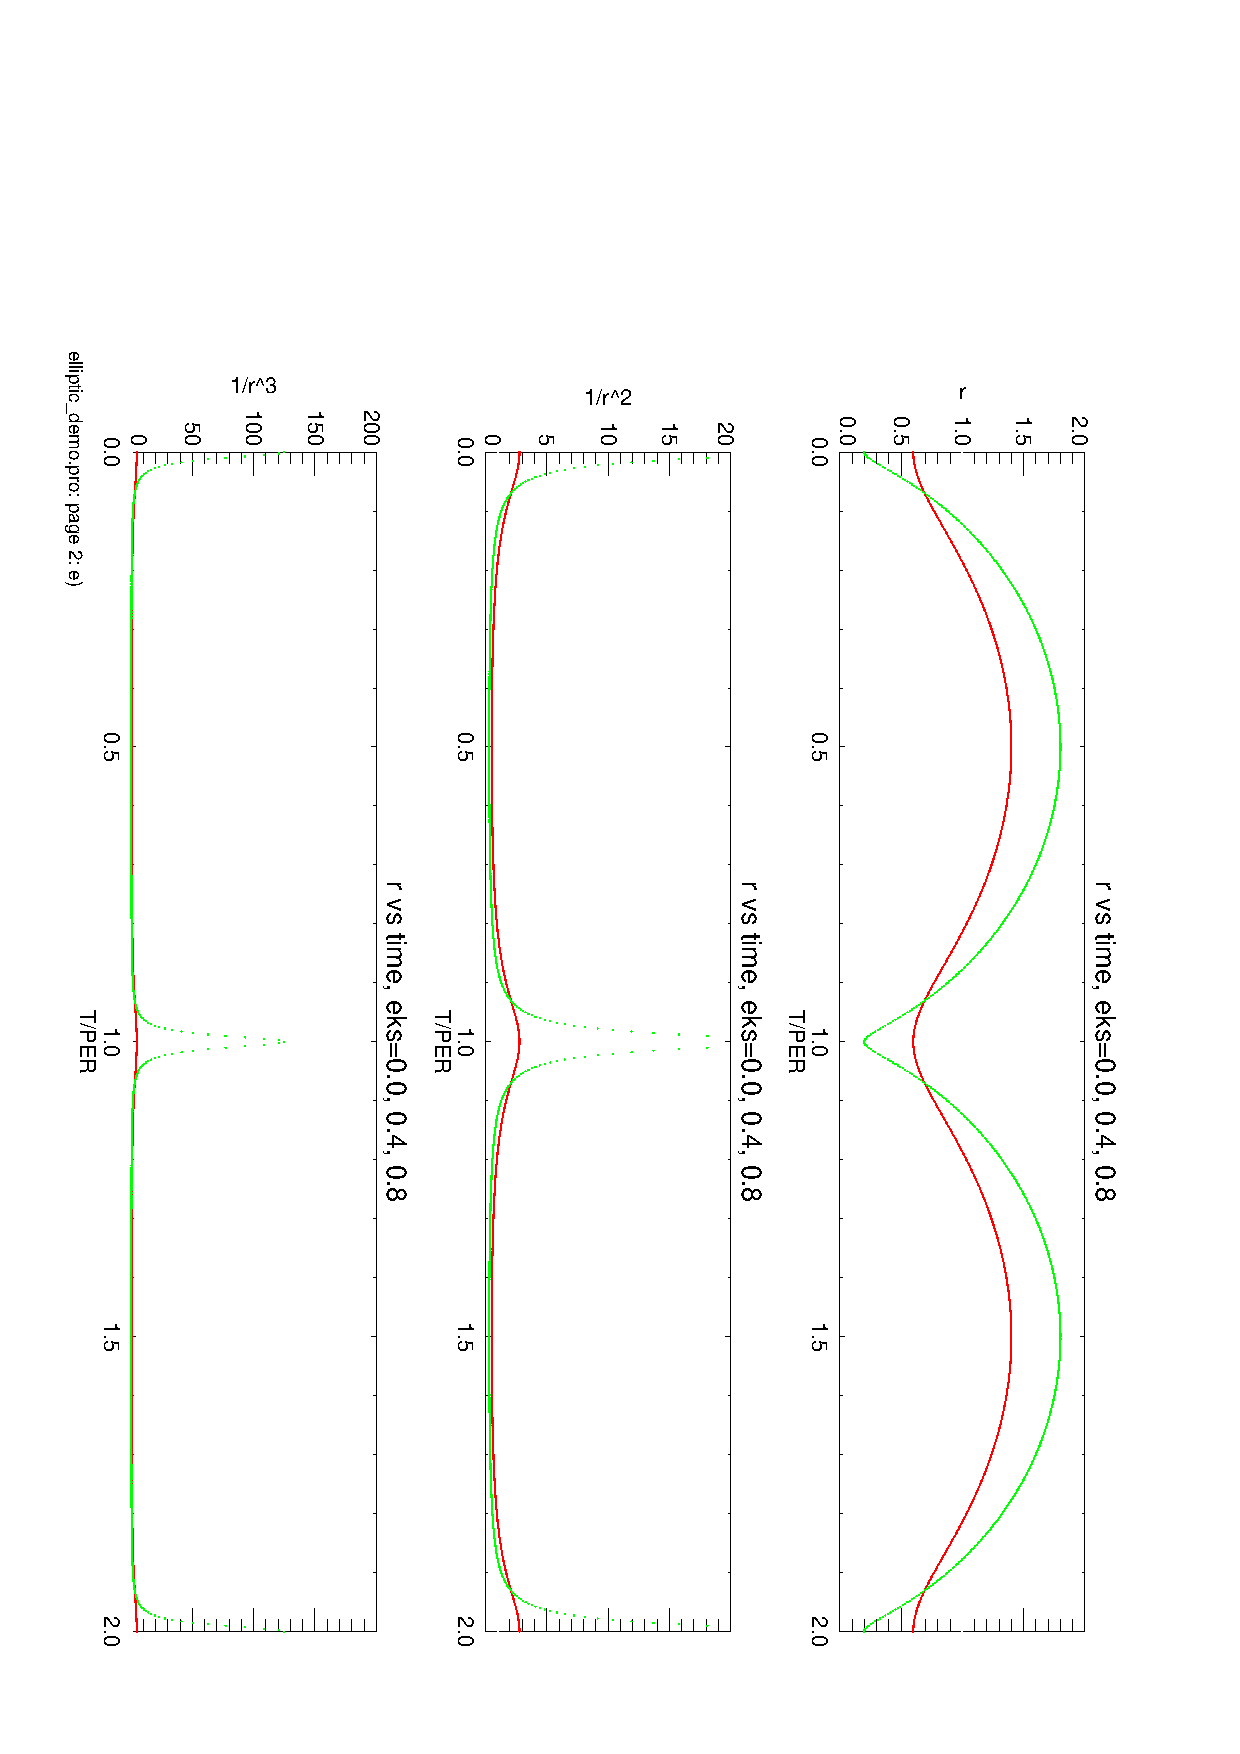
\includegraphics[width=0.9\paperwidth]{elliptic_demo_2.pdf}
\clearpage

%********************************************************

{\red \scriptsize
\begin{verbatim}

;----------------------------------------------
; f) PLOT vr,vt,v vs. TIME
;----------------------------------------------
;choose \mu=G(m1+m2) = 1 -> orbital period = 2\pi

myy=1.
a=1.
vcirc=sqrt(myy/a)

!p.multi=[0,1,3]
nwin
!p.charsize=2.
;eccentricity values
  eks_tab=[0., 0.4, 0.8]
  M=findgen(201)/100.*2.*!dpi

;---------- 
; plot v(t)
;---------- 
  for i=0,n_elements(eks_tab)-1 do begin
    eks=eks_tab(i)
    b=sqrt(1.-eks^2)*a
    e=m*0
    for j=0,n_elements(m)-1 do begin
      kepler,m(j),eks,eano
      e(j)=eano
    endfor
    xx=a*(cos(e)-eks)
    yy=b*sin(e)
    ep=sqrt(myy/a^3)/(1-eks*cos(e))
    vx=-a*sin(e)*ep
    vy= b*cos(e)*ep

;numerical velocity components
    vr=(vx*xx+vy*yy)/sqrt(xx^2+yy^2)
    vtx=vx-vr*xx/sqrt(xx^2+yy^2)
    vty=vy-vr*yy/sqrt(xx^2+yy^2)
    vt=sqrt(vtx^2+vty^2)	
    v=sqrt(vx^2+vy^2)

;analytic velocity components
    rr=a*(1-eks*cos(e))    
    vr_ana=vcirc*a/rr*eks*sin(e)
    vt_ana=vcirc*b/rr
    v_ana =vcirc*sqrt((1+eks*cos(e))/(1-eks*cos(e)))
	
    if(i eq 0) then begin
      plot,m/2/!pi,v,xtitle='T/PER',ytitle='v',$
           xrange=[0,2],yrange=[0,4],$
           xs=1,ys=1,title='eks=0.0, 0.4, 0.8: symbol=numerical',psym=6,syms=.4
      oplot,m/2/!pi,v_ana,lines=0        
    endif
    oplot,m/2/!pi,v,col=i+2,psym=6,syms=.4
      oplot,m/2/!pi,v_ana,lines=0,col=i+2        
  endfor

;---------- 
; plot v_r(t)
;---------- 
  for i=0,n_elements(eks_tab)-1 do begin
    eks=eks_tab(i)
    b=sqrt(1.-eks^2)*a
    e=m*0
    for j=0,n_elements(m)-1 do begin
      kepler,m(j),eks,eano
      e(j)=eano
    endfor
    xx=a*(cos(e)-eks)
    yy=b*sin(e)
    ep=sqrt(myy/a^3)/(1-eks*cos(e))
    vx=-a*sin(e)*ep
    vy= b*cos(e)*ep

;numerical velocity components
    vr=(vx*xx+vy*yy)/sqrt(xx^2+yy^2)
    vtx=vx-vr*xx/sqrt(xx^2+yy^2)
    vty=vy-vr*yy/sqrt(xx^2+yy^2)
    vt=sqrt(vtx^2+vty^2)	
    v=sqrt(vx^2+vy^2)

;analytic velocity components
    rr=a*(1-eks*cos(e))    
    vr_ana=vcirc*a/rr*eks*sin(e)
    vt_ana=vcirc*b/rr
    v_ana =vcirc*sqrt((1+eks*cos(e))/(1-eks*cos(e)))
	
    if(i eq 0) then begin
      plot,m/2/!pi,vr,xtitle='T/PER',ytitle='v_r',$
           xrange=[0,2],yrange=[-2,2],$
           xs=1,ys=1,title='eks=0.0, 0.4, 0.8: symbol=numerical',psym=6,syms=.4
      oplot,m/2/!pi,vr_ana,lines=0        
    endif
    oplot,m/2/!pi,vr,col=i+2,psym=6,syms=.4
      oplot,m/2/!pi,vr_ana,lines=0,col=i+2        
  endfor


;---------- 
; plot v_t(t)
;---------- 
  for i=0,n_elements(eks_tab)-1 do begin
    eks=eks_tab(i)
    b=sqrt(1.-eks^2)*a
    e=m*0
    for j=0,n_elements(m)-1 do begin
      kepler,m(j),eks,eano
      e(j)=eano
    endfor
    xx=a*(cos(e)-eks)
    yy=b*sin(e)
    ep=sqrt(myy/a^3)/(1-eks*cos(e))
    vx=-a*sin(e)*ep
    vy= b*cos(e)*ep

;numerical velocity components
    vr=(vx*xx+vy*yy)/sqrt(xx^2+yy^2)
    vtx=vx-vr*xx/sqrt(xx^2+yy^2)
    vty=vy-vr*yy/sqrt(xx^2+yy^2)
    vt=sqrt(vtx^2+vty^2)	
    v=sqrt(vx^2+vy^2)

;analytic velocity components
    rr=a*(1-eks*cos(e))    
    vr_ana=vcirc*a/rr*eks*sin(e)
    vt_ana=vcirc*b/rr
    v_ana =vcirc*sqrt((1+eks*cos(e))/(1-eks*cos(e)))
	
    if(i eq 0) then begin
      plot,m/2/!pi,vt,xtitle='T/PER',ytitle='v_t',$
           xrange=[0,2],yrange=[0,4],$
           xs=1,ys=1,title='eks=0.0, 0.4, 0.8: symbol=numerical',psym=6,syms=.4
      oplot,m/2/!pi,vt_ana,lines=0        
    endif
    oplot,m/2/!pi,vt,col=i+2,psym=6,syms=.4
      oplot,m/2/!pi,vt_ana,lines=0,col=i+2        
  endfor

;**********************************************************
 xyouts,0.01,0.01,'elliptic_demo.pro: page 3: f)',/normal,chars=.75
 !p.multi=0
 !p.charsize=1.
 charsize,1
;**********************************************************
\end{verbatim}}

\black

\vspace{-12cm}
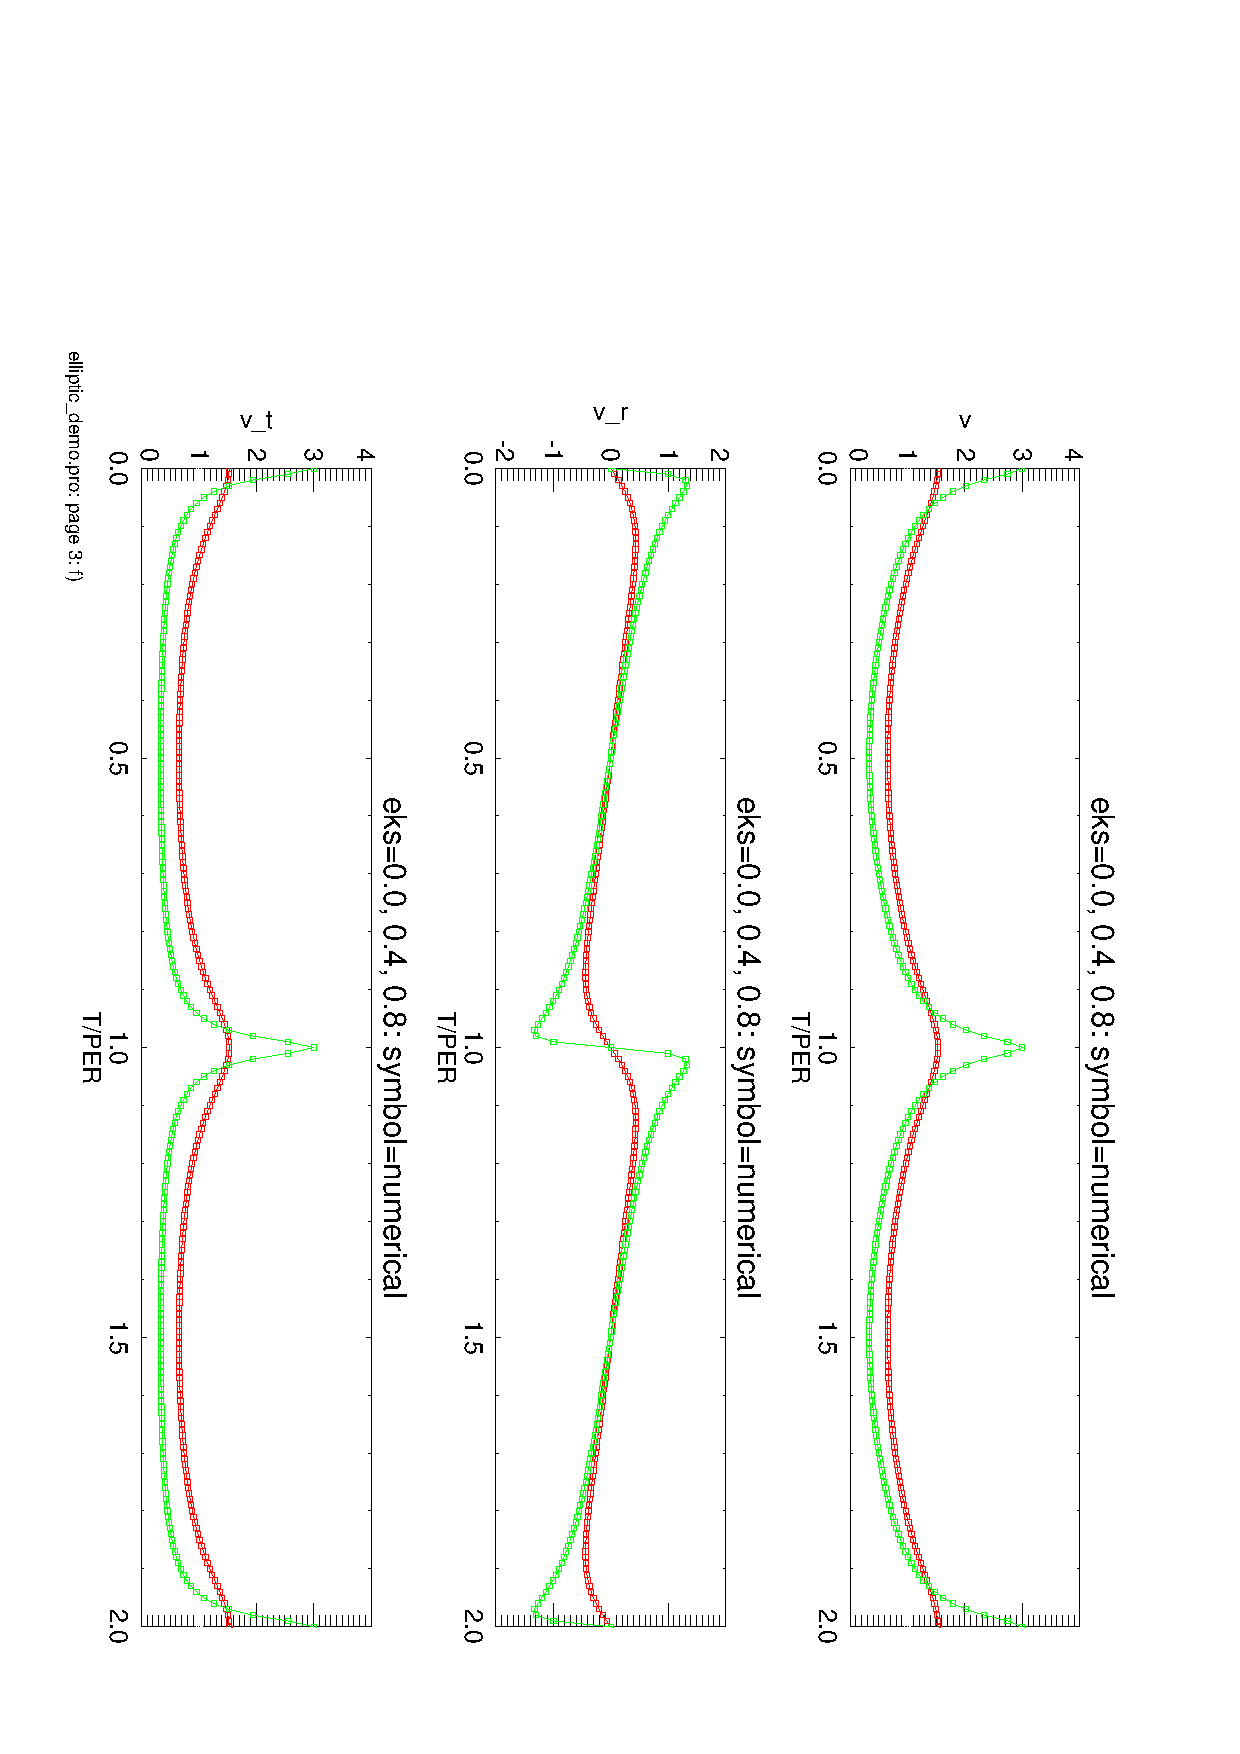
\includegraphics[width=0.9\paperwidth]{elliptic_demo_3.pdf}
\clearpage
%********************************************************
{\red \scriptsize \begin{verbatim}
;----------------------------------------------
; g) PLOT EKIN, EPOT, H vs TIME
;----------------------------------------------
;choose \mu=G(m1+m2) = 1 -> orbital period = 2\pi

myy=1.
a=1.
vcirc=sqrt(myy/a)
!p.multi=0
nwin
!p.charsize=1.

;eccentricity values
  eks_tab=[0., 0.4, 0.8]
  M=findgen(201)/100.*2.*!dpi

  for i=0,n_elements(eks_tab)-1 do begin
    eks=eks_tab(i)
    b=sqrt(1.-eks^2)*a
    e=m*0

    for j=0,n_elements(m)-1 do begin
      kepler,m(j),eks,eano
      e(j)=eano
    endfor

    rr=a*(1-eks*cos(e))    
    vr_ana=vcirc*a/rr*eks*sin(e)
    vt_ana=vcirc*b/rr
    v_ana =vcirc*sqrt((1+eks*cos(e))/(1-eks*cos(e)))	
    ekin=0.5*v_ana^2
    epot=-myy/rr   	
    amom=rr*vt_ana
 
    print,'ECCENTRICITY, ANGULAR MOMENTUM',eks,mean(amom)

    if(i eq 0) then begin
      plot,m/2/!pi,EKIN,xtitle='T/PER',ytitle='EKIN, EPOT, H, A_MOM',$
           xrange=[0,2],yrange=[-2,2],$
           xs=1,ys=1,title='eks=0.0, 0.4, 0.8'
      oplot,m/2/!pi,EPOT
      xyouts,0.75,-1.5,'EPOT'
      xyouts,0.75, 1.5,'EKIN'
      xyouts,1.,-.4,'ETOT=-0.5'
    endif

    oplot,m/2/!pi,EKIN,col=i+2
      oplot,m/2/!pi,EPOT,lines=0,col=i+2
      oplot,m/2/!pi,epot+ekin,col=i+2,lines=2        
      oplot,m/2/!pi,amom,col=i+2,lines=1
      ff='(f6.3)'
      xyouts,1.15,mean(amom)+.01,col=i+2,string(eks,ff)+' -> AMOM='+string(mean(amom),ff)
  endfor

;**********************************************************
 xyouts,0.01,0.01,'elliptic_demo.pro: page 4: g)',/normal,chars=.75
 !p.multi=0
 !p.charsize=1.
;**********************************************************
end

\end{verbatim}} \black
\newpage
.

\vspace{-15cm}

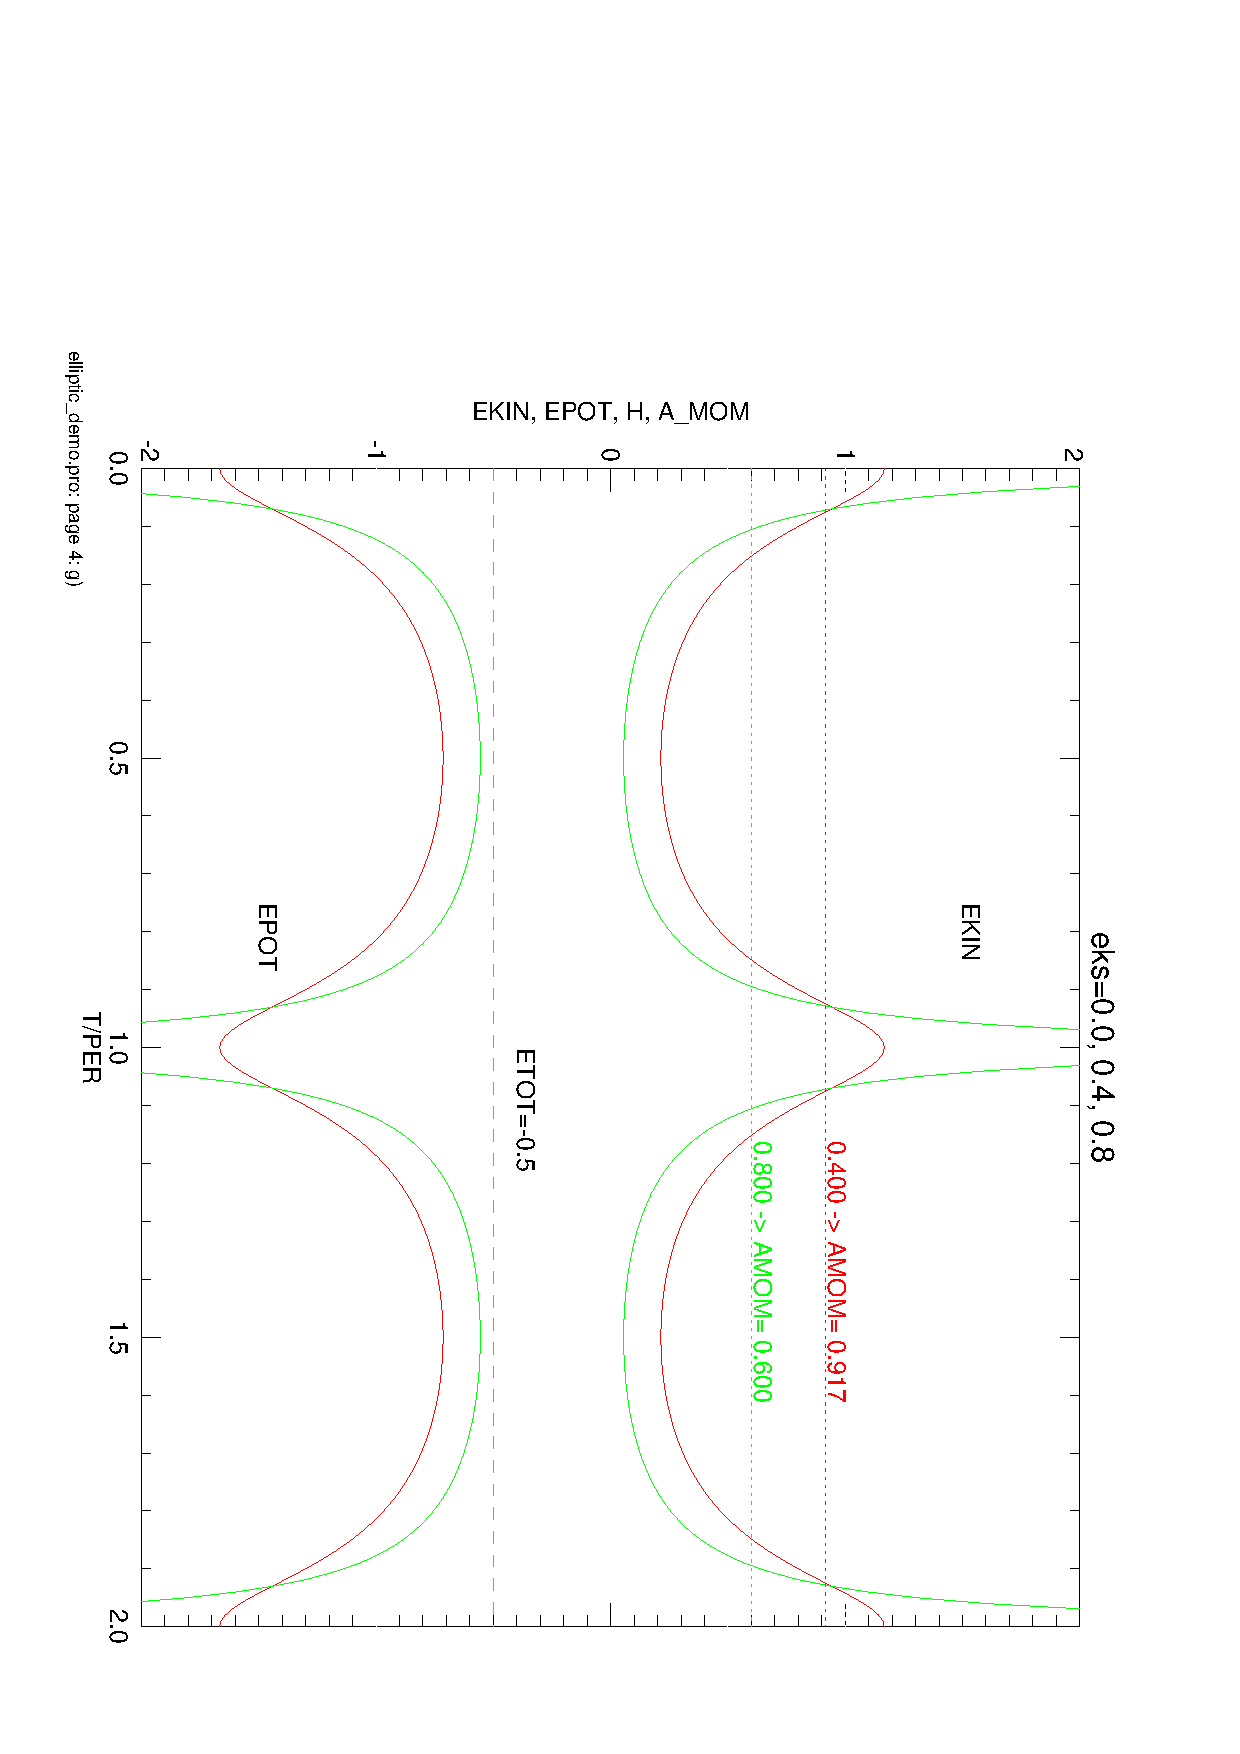
\includegraphics[width=0.9\paperwidth,height=1\paperheight]{elliptic_demo_4.pdf}

\clearpage
\newpage
\black

{\isob 3. Compare different anomalies: $E$, $f$, $M$} \ \small \framebox{ano\_demo.pro}


%********************************************************
{\red \scriptsize \begin{verbatim}

;**********************************************
;ano_demo.pro
;study elliptic orbit
;HS 2002/1.11.2006
;**********************************************

program='ano_demo'
ps=0
psdirect,program,ps,/color

!p.multi=[0,2,2]
!p.charsize=0.7
col1=1
if(!d.name eq 'PS') then col1=0
;*************************************
;compare 
; mean anomaly M
; eccentric anomaly E
; true anomaly f
;*************************************

  a=1.
  eks=.5         ;try different values !!
  
;evaluate M with npoints values
  npoints=50
  M=findgen(npoints)*2.*!dpi/npoints

;solve E from Kepler's equation
  e=m*0
  for j=0,n_elements(m)-1 do begin
      kepler,m(j),eks,eano
      e(j)=eano
  endfor
  
;solve f from E
  sine=sin(e)
  cose=cos(e)
  cosf=(cose-eks)/(1.-eks*cose)
  sinf=sqrt(1.-eks^2)*sine/(1.-eks*cose)
  f=atan(sinf,cosf)
  index=where(f lt 0,count)
  if(count ge 1) then f(index)=f(index)+2.*!pi

;************************
;plot M,E,F
;************************
 nwin
  plot,m*!radeg,m*!radeg,lines=2,xr=[0,360],xs=1,yr=[0,360],ys=1,$
    xtitle='M Mean anomaly',ytitle='E, f',$
    title='eccentricity='+string(eks,'(f8.3)'),col=col1
  oplot,m*!radeg,f*!radeg,col=2,lines=1
  oplot,m*!radeg,e*!radeg,col=3

  plots,[15,40],[320,320],col=3
  plots,[15,40],[290,290],col=2,lines=1
  plots,[15,40],[260,260],col=col1,lines=2
  xyouts,50,320,'eccentric anomaly E',col=3
  xyouts,50,290,'true anomaly f',col=2
  xyouts,50,260,'mean anomaly M',col=col1

;************************
;plot f-M, E-M
;************************
nwin
  plot,m*!radeg,(f-M)*!radeg,xr=[0,360],yr=[-1,1]*eks*3*!radeg,xs=1,$
       xtitle='M Mean anomaly',ytitle='f-M and E-M',$
       title='eccentricity='+string(eks,'(f8.3)'),col=2,lines=1
  oplot,m*!radeg,(E-M)*!radeg,col=3

;************************
;f-M series
;************************
nwin

  plot,m*!radeg,(f-M)*!radeg,psym=6,xr=[0,360],yr=[-1,1]*eks*3*!radeg,xs=1,$
       xtitle='M Mean anomaly',ytitle='f-M',$
       title='eccentricity='+string(eks,'(f8.3)'),col=col1,syms=.25

 term1=2*eks*sin(m)
 term2=5./4.*eks^2*sin(2*m)
 term3=(13./12.*sin(3*m)-0.25*sin(m))*eks^3

       oplot,m*!radeg,term1*!radeg,lines=1,col=2
       oplot,m*!radeg,(term1+term2)*!radeg,lines=2,col=3
       oplot,m*!radeg,(term1+term2+term3)*!radeg,lines=0,col=5

dy=   3*eks*!radeg*.3
      xyouts,10,-1*dy,'  2*eks*sin(m)',col=2,chars=0.7
      xyouts,10,-2*dy,'+ 5/4*eks^2*sin(2*m)',col=3,chars=0.7
      xyouts,10,-3*dy,'+ (13./12.*sin(3*m)-0.25*sin(m))*eks^3',$
             col=5,chars=0.7

;************************
;e-M series
;************************
nwin
  plot,m*!radeg,(e-M)*!radeg,psym=6,xr=[0,360],yr=[-1,1]*eks*2*!radeg,xs=1,$
       xtitle='M Mean anomaly',ytitle='e-M',$
       title='eccentricity='+string(eks,'(f8.3)'),col=col1,syms=.25

 term1=eks*sin(m)
 term2=1./2.*eks^2*sin(2*m)
 term3=(3./8.*sin(3*m)-1./8*sin(m))*eks^3

       oplot,m*!radeg,term1*!radeg,lines=1,col=2
       oplot,m*!radeg,(term1+term2)*!radeg,lines=2,col=3
       oplot,m*!radeg,(term1+term2+term3)*!radeg,lines=0,col=5

dy=   3*eks*!radeg*.2
       xyouts,10,-1*dy,'  eks*sin(m)',col=2,chars=0.7
       xyouts,10,-2*dy,'+ 1/2*eks^2*sin(2*m)',col=3,chars=0.7
       xyouts,10,-3*dy,'+ (3./8.*sin(3*m)-1./8*sin(m))*eks^3',col=5,$
              chars=0.7

xyouts,0.01,0.01,'ano_demo.pro',chars=0.75,/normal
!p.multi=0
psdirect,program,ps,/stop
end
\end{verbatim}} \black
\newpage
.

\vspace{-15cm}

\includegraphics[width=0.9\paperwidth,height=1\paperheight]{ano_demo.pdf}

\clearpage




\newpage

\black
{\isob 4. Numerical evaluation of time averages} \ \small \framebox{aver\_demo.pro}

%********************************************************
{\red \scriptsize \begin{verbatim}


;**********************************************
;aver_demo.pro
;study elliptic orbit
;HS 05.11.02/01.11.2006
;**********************************************

program='aver_demo'
ps=0
psdirect,program,ps,/color


;*********************************************
;calculate time-averages of <r>, <1/r> , <v^2>
;also <1/r^2>,<1/r^3>,<r^2>
;*************************************
;with eccentricity 0.1,0.2,...,0.8
;choose a=1. semimajor axis
;myy=1   G*(m1+m2)
;*************************************
   a=1.
   myy=1.

;eccentricity values
   eks_tab=findgen(21)/20.*.8

;store averages to
   r_tab   = eks_tab*0.
   r2_tab  = eks_tab*0.
   rm1_tab = eks_tab*0.
   rm2_tab = eks_tab*0.
   rm3_tab = eks_tab*0.
   v2_tab  = eks_tab*0.
   vm1_tab  = eks_tab*0.
   
;evaluate with npoints values of time (or M)
   npoints=200
   M=findgen(npoints)*2.*!dpi/npoints
   
;requires solution of eccentric anomaly from Kepler's equation
;M = E - eks*sin(E)
   
   for i=0,n_elements(eks_tab)-1 do begin       
       eks=eks_tab(i)
       b=sqrt(1.-eks^2)*a
       e=m*0
       for j=0,n_elements(m)-1 do begin
           kepler,m(j),eks,eano
           e(j)=eano
       endfor
       
       sine=sin(e)
       cose=cos(e)
       xx=a*(cose-eks)
       yy=b*sine
       dedt=sqrt(myy/a^3)/(1.d0-eks*cos(e))
       vxx=-a*sine*dedt
       vyy=b*cose*dedt
       
       r=sqrt(xx^2+yy^2)
       v=sqrt(vxx^2+vyy^2)
; or v=sqrt(myy/a)*sqrt((1.+eks*cose)/(1.-eks*cose))
       
       r_tab(i)=mean(r)
       r2_tab(i)=mean(r^2)
       rm1_tab(i)=mean(1./r)
       rm2_tab(i)=mean(1./r^2)
       rm3_tab(i)=mean(1./r^3)
       v2_tab(i)=mean(v^2)
       vm1_tab(i)=mean(1./v)
   endfor
   

   
   nwin
   !p.multi=[0,3,2]
   !p.charsize=1.2
   
   
   plot,eks_tab,r2_tab,xtitle='eks',ytitle='<r^2>/a',$
     title='npoints='+string(npoints,'(i6)')
   oplot,eks_tab,(1.+3*eks_tab^2/2),psym=6,col=2
   
   plot,eks_tab,r_tab,xtitle='eks',ytitle='<r>/a',title='symbol=analytical'
   oplot,eks_tab,(1.+eks_tab^2/2),psym=6,col=2
   
   plot,eks_tab,rm1_tab,xtitle='eks',ytitle='<1/r>/a',yr=[0,1.2]
   oplot,eks_tab,1.+eks_tab*0,psym=6,col=2
   
   plot,eks_tab,rm2_tab,xtitle='eks',ytitle='<1/r^2>/a'
   oplot,eks_tab,(1.-eks_tab^2)^(-0.5),psym=6,col=2
   
   plot,eks_tab,rm3_tab,xtitle='eks',ytitle='<1/r^3>/a'
   oplot,eks_tab,(1.-eks_tab^2)^(-1.5),psym=6,col=2

   plot,eks_tab,v2_tab,xtitle='eks',ytitle='<v^2>/(myy/a)',yr=[0,1.2]
   oplot,eks_tab,1.+eks_tab*0,psym=6,col=2
   
   xyouts,0.01,0.01,/normal,'aver_demo.pro',chars=.75
   charsize,1
   !p.multi=0


psdirect,program,ps,/color,/stop

end


\end{verbatim}} \black
\newpage
.

\vspace{-15cm}

\includegraphics[width=0.9\paperwidth,height=1\paperheight]{aver_demo.pdf}

\clearpage


%-------------------------------------------------------------------------



\end{document}









